\documentclass{article}
\usepackage{unipr_org_notes}
% grafici
\usepackage{pgfplots}
\usepackage{float}


\renewcommand{\coursetitle}{Analisi statica e verifica del software}

% \addauthor{Nome}{Mail}


\renewcommand{\authorname}{Simone Colli\\ Manuel Di Agostino}
% \renewcommand{\authoremail}{simone.colli@studenti.unipr.it\\  manuel.diagostino@studenti.unipr.it}

\renewcommand{\notedate}{%
    Appunti del corso tenuto dal \textbf{Prof. Vincenzo Arceri} \\
    \medskip % Aggiunge un piccolo spazio verticale
    Università degli Studi di Parma \\
    Anno Accademico 2025/2026
}


\begin{document}
\maketitle

\tableofcontents

\section{Introduzione}

\subsection{Cos'è l'affidabilità del software?}

\begin{definizione}{Affidabilità del Software (IEEE 610.12\-1990)}{ieee610121990}
"The ability of a system or component to perform its required functions
under stated conditions for a specified period of time"

Ovvero:

"La capacità di un sistema o componente di eseguire le funzioni richieste
in condizioni specificate per un periodo di tempo specificato"
\end{definizione}

\begin{definizione}{Gestione dell'Affidabilità del Software (IEEE 982.1\-1988)}{ieee98211888}
"The process of optimizing the reliability of software through a program that
emphasizes software error prevention, fault detection and removal, and the
use of measurements to maximize reliability in light of project constraints
such as resources, schedule and performance"

Ovvero:

"Il processo di ottimizzazione dell'affidabilità del software attraverso un
programma che enfatizza la prevenzione degli errori software, il rilevamento
e la rimozione dei guasti, e l'uso di misurazioni per massimizzare l'affidabilità
alla luce dei vincoli del progetto come risorse, tempi e prestazioni"

\end{definizione}

Sfruttando le definizioni \ref{def:ieee610121990} e \ref{def:ieee98211888},
è possibile riassumere che l'affidabilità del software consiste in 3 attività:
\begin{itemize}
    \item Prevenzione degli errori.
    \item Rilevamento e rimozione dei guasti.
    \item Valutazione per massimizzare l'affidabilità, in particolare valutazioni
    a supporto delle prime due attività.
\end{itemize}

\subsection{Perché l'affidabilità del software è importante?}

L'importanza dell'affidabilità del software deriva dalle enormi conseguenze
economiche e operative che i bug possono causare.

Alcune stime indicano che:
\begin{itemize}
    \item I bug nei software costano circa \(60\) miliardi di dollari all'anno
    negli Stati Uniti.
    \item L'economia mondiale perde circa \(250\) miliardi di dollari all'anno
    a causa di qualsiasi tipo di attacco palese (overt attack).
    \item I difetti nel software rendono la programmazione molto dolorosa.
\end{itemize}

Alcuni esempi di fallimenti dovuti a bug software includono:
\begin{itemize}
    \item Il disastro del volo 501 di Ariane 5 nel 1996, che è esploso dopo 37 secondi
    dal decollo a causa di un errore di overflow durante la conversione da un float 64 bit ad un intero 16 bit.
    Questo evento ha causato una perdita di circa \(370.000.000\) dollari.
    \item Il bug del Pentium FDIV nel 1994, che ha causato errori di calcolo
    nelle divisioni in virgola mobile. Questo bug ha portato a una perdita di
    circa \(475.000.000\) dollari.
    \item L'aggiornamento difettoso di CrowdStrike nel 2024, che ha causato
    più di \(5000\) voli cancellati. Questo evento ha impattato su banche,
    governi e infrastrutture critiche. Le perdite economiche sono state
    stimate a circa \(5.400.000.000\) dollari.
\end{itemize}

La lista di esempi potrebbe continuare, ma l'importante è comprendere
che l'affidabilità del software è cruciale per evitare perdite economiche
significative e garantire il corretto funzionamento dei sistemi.

\subsection{Validazione e Verifica}

La validazione e la verifica sono due processi distinti ma complementari
nell'ambito dello sviluppo del software, entrambi mirati a garantire che
il software soddisfi i requisiti e funzioni correttamente.


La \textbf{validazione} si concentra sulla domanda: "Stiamo costruendo il
prodotto giusto?".
Essa verifica che il software soddisfi le esigenze e le aspettative degli
utenti finali.
La \textbf{verifica}, d'altra parte, si concentra sulla domanda: "Stiamo
costruendo il prodotto nel modo giusto?".
Essa assicura che il software sia sviluppato correttamente secondo le
specifiche tecniche e i requisiti di progetto.


\begin{figure}[H]
    \centering
    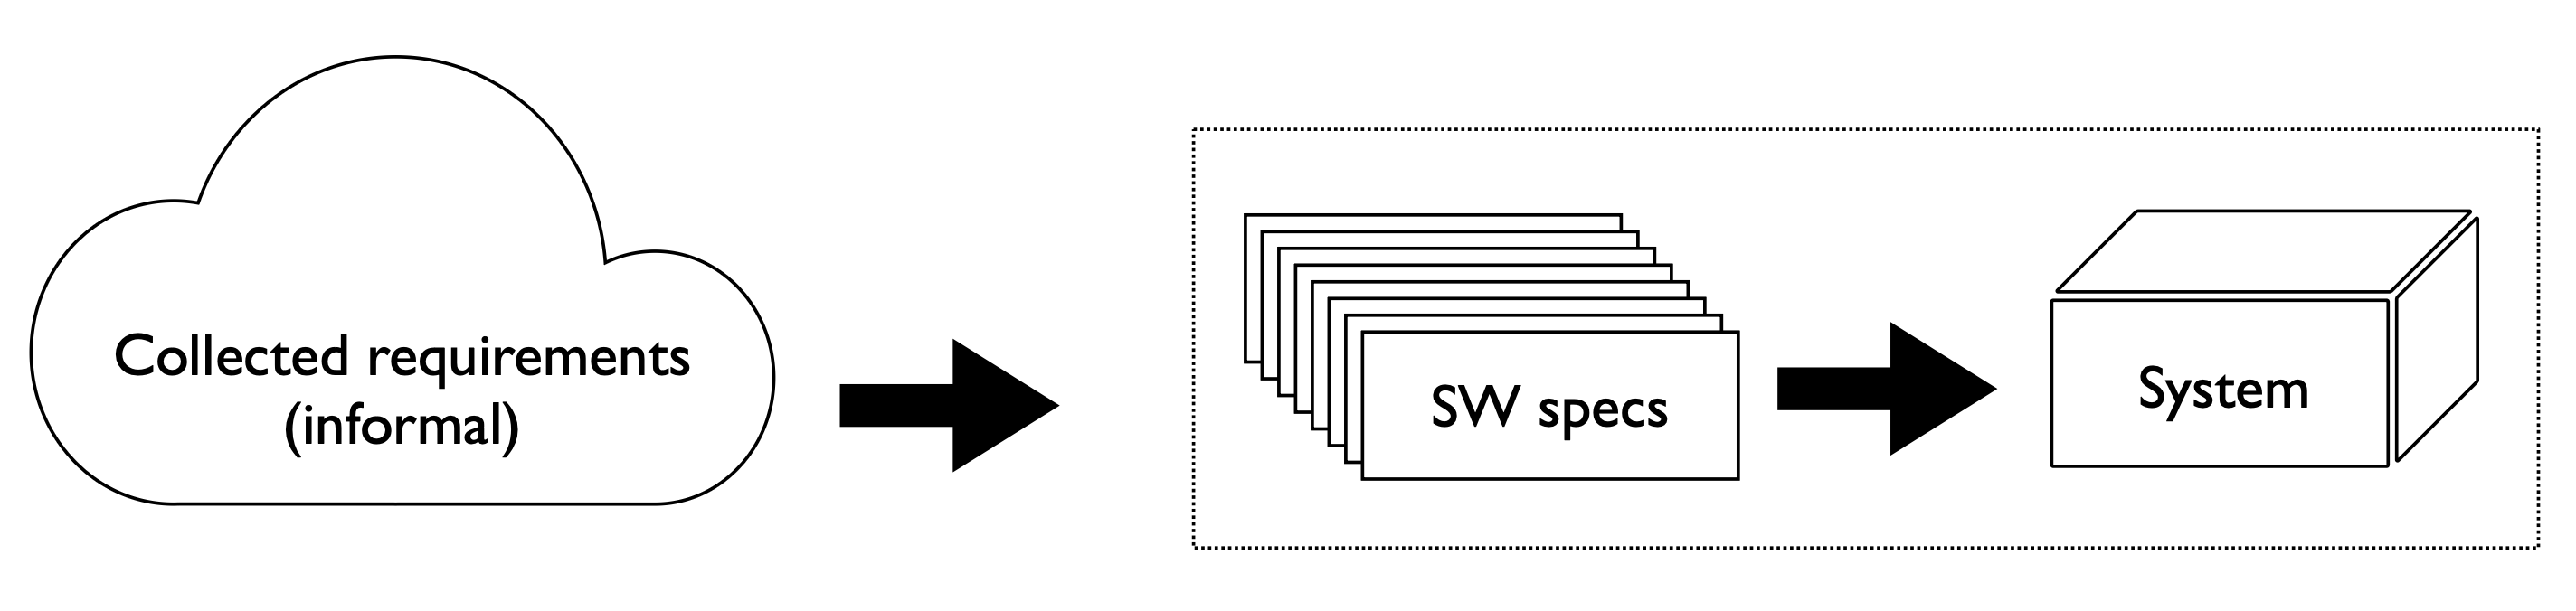
\includegraphics[width=0.8\textwidth]{images/th_01/01.png}
    \caption{L'immagine illustra la differenza tra validazione e verifica.}
    \label{fig:th_01_01}
\end{figure}

\begin{esempio}{Risposta dell'ascensore}{elevator_response}

Un esempio pratico di validazione e verifica può essere trovato nel
comportamento di un sistema di risposta dell'ascensore.

Una specifica validabile ma non verificabile potrebbe essere:
"Se un utente preme il pulsante di richiesta a un piano $i$, un ascensore
disponibile deve arrivare al piano $i$ entro un tempo ragionevole".

Una specifica verificabile è:
"Se un utente preme il pulsante di richiesta a un piano $i$, un ascensore
disponibile deve arrivare al piano $i$ entro 30 minuti".

\end{esempio}

\subsection{Verifica del Software}

Lo scopo della verifica del software è verificare alcune affermazioni di
correttezza riguardante un programma:
\begin{itemize}
    \item La \textbf{correttezza funzionale}, ovvero che il programma
    soddisfi i requisiti funzionali specificati.
    \item L'\textbf{assenza di errori non funzionali} (non cosa fa il
    programma, ma come lo fa), come ad esempio: soddisfacimento di vincoli
    spaziali e/o temporali, assenza di errori a runtime, soddisfacimento di
    vincoli di sicurezza, ecc.
\end{itemize}

\section*{Bad news: there’s no silver bullet}

Non esiste un metodo di verifica che sia contemporaneamente:
\begin{itemize}
    \item \textbf{Automatico}: non richiede interazione umana.
    \item \textbf{Potente}: è in grado di dimostrare proprietà non banali (\emph{non-trivial properties}).
    \item \textbf{Corretto (Sound)}: non dimostra mai una proprietà se questa non è vera.
    \item \textbf{Completo (Complete)}: dimostra sempre la proprietà se essa è vera e non fallisce mai nel dichiarare la correttezza di un programma corretto.
\end{itemize}

Il \textbf{teorema di Rice} afferma che tutte le proprietà non banali del
comportamento di un programma scritto in un linguaggio di programmazione
Turing-completo sono indecidibili.
L'\textbf{indecidibilità} di una proprietà implica che non esiste alcun metodo
di verifica automatico che sia allo stesso tempo \textbf{corretto} e
\textbf{completo}.
\section{Background matematico}
Per poter discutere in modo rigoroso di tecniche di verifica del software,
è necessario introdurre alcuni concetti matematici di base relativi alla
teoria della computazione e alla logica formale.

\subsection{Set notation}
\subsection{Partial order}
\subsection{Powerset}
\subsection{Diagramma di Hasse}
\subsection{Upper e lower bounds}
\subsection{Lattice}




\end{document}